\documentclass[11pt]{article}
\usepackage[utf8]{inputenc}
\usepackage[a4paper,margin=0.8in]{geometry}
\usepackage{amsmath,amssymb}
\usepackage{hyperref}
\usepackage{enumitem}
\usepackage{titlesec}
\usepackage{xcolor}
\usepackage{fancyhdr}
\usepackage{tikz}
\usepackage{graphicx}
\usepackage{eso-pic}

\graphicspath{{../}}

\definecolor{kcpc-text}{RGB}{20,20,20}
\definecolor{kcpc-muted}{RGB}{90,90,90}
\definecolor{kcpc-red}{RGB}{176,0,0}

\pagestyle{fancy}
\fancyhf{}
\lhead{\textcolor{kcpc-text}{\small\bfseries Reading}}
\rhead{\textcolor{kcpc-muted}{\small Week 4}}
\cfoot{\textcolor{kcpc-muted}{\small KCPC}}
\renewcommand{\headrulewidth}{0.4pt}
\renewcommand{\headrule}{\hbox to\headwidth{\color{kcpc-red}\leaders\hrule height \headrulewidth\hfill}}
\renewcommand{\footrulewidth}{0pt}
\setlength{\headheight}{28pt}

\AddToShipoutPictureBG{%
    \begin{tikzpicture}[remember picture,overlay]
        \node[opacity=0.035, at=(current page.center)]
        {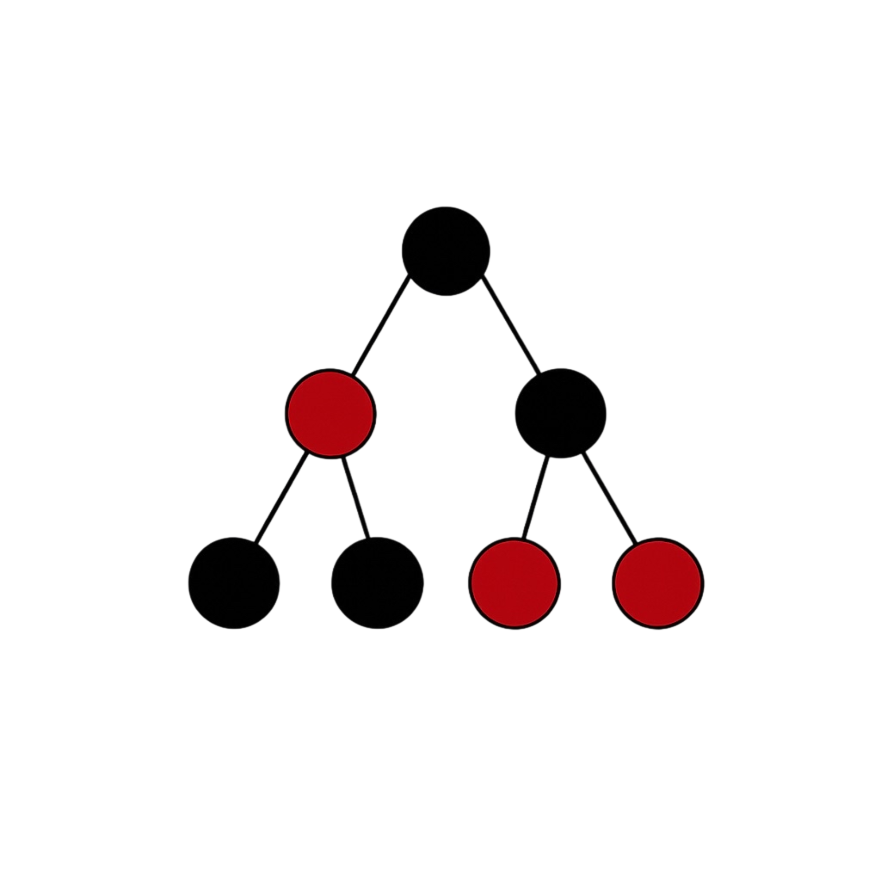
\includegraphics[width=0.38\paperwidth]{kcpc-logo.png}};
    \end{tikzpicture}%
}

\titleformat{\section}{\large\bfseries\color{kcpc-red}}{}{0pt}{}
\setlist[itemize]{noitemsep, topsep=4pt}
\setlist[enumerate]{noitemsep, topsep=4pt}

\hypersetup{
    colorlinks=true,
    linkcolor=kcpc-red,
    urlcolor=kcpc-red
}

\title{KCPC Week 4 Reading\\Introduction to Graphs: Traversals, Structure, and Modelling}
\author{}
\date{}

\begin{document}

\maketitle
\thispagestyle{fancy}

\noindent
Follow this location-stamped reading guide alongside the Workshop 4 slides and problem sheet. Each entry attributes the reference, specifies the exact chapters, sections, and page numbers covering the workshop's theory, and connects each reading directly to the corresponding problems. For primary historical and research literature, see \emph{Week 4 Papers}.

\section*{I. Core Competitive Programming Textbooks}

\subsection*{Competitive Programmer's Handbook (Antti Laaksonen)}
Draft of July 3, 2018 (freely available online). \url{https://cses.fi/book/book.pdf}

\begin{itemize}
    \item \textbf{Chapter 11: Basics of Graphs (\S\S 11.1--11.4, pp.~109--116):}
    Introduces graph terminology (paths, cycles, connectivity, connected components, trees, directed vs.\ undirected graphs, vertex degrees, and bipartite colourings) and compares adjacency list ($O(V + E)$), adjacency matrix ($O(V^2)$), and edge list representations. Read this alongside Slide Sections 1--2.
    \item \textbf{Chapter 12: Graph Traversal (\S\S 12.1--12.2, pp.~117--124):}
    Covers Depth-First Search (DFS), Breadth-First Search (BFS), shortest unweighted path computation, connected component enumeration, undirected cycle detection via edge/degree analysis, and bipartiteness testing (2-colouring). Directly supports Warm-Up Problems 1.1--1.4 (\emph{Building Roads}, \emph{Message Route}, \emph{Round Trip}, \emph{Building Teams}) and Core Problem 2.2 (\emph{Cyclic Components}).
    \item \textbf{Chapter 14: Tree Algorithms (\S\S 14.1--14.2, pp.~133--138):}
    Develops tree traversal properties and presents Algorithm 2 (\S 14.2, pp.~136--137): computing the diameter of a tree using two BFS/DFS traversals by finding the farthest node from an arbitrary root. Directly supports Problem 2.5 (\emph{Tree Diameter}).
    \item \textbf{Chapter 16: Directed Graphs (\S\S 16.1--16.3, pp.~151--158):}
    Covers topological sorting on Directed Acyclic Graphs (DAGs), dynamic programming on DAGs (counting the number of paths and finding longest/shortest paths), and successor/functional graphs in which every vertex has out-degree $1$. Directly supports Problems 2.1, 2.3, 2.4, and 3.2 (\emph{Badge}, \emph{DAG Number of Routes}, \emph{Longest Path}, and \emph{Game on Axis}).
\end{itemize}

\subsection*{Competitive Programming 4, Book 1 (Steven Halim, Felix Halim, Suhendry Effendy)}
Lulu Press / NUS, 2020. \url{https://cpbook.net/}

\begin{itemize}
    \item \textbf{Chapter 4: Graph (\S\S 4.1--4.2, pp.~169--192):}
    Provides concrete C++ and Python implementations of graph data structures, DFS, BFS, connected components, flood fill, topological sort (both DFS post-order and Kahn's algorithm), bipartite graph check, and cycle detection on directed and undirected graphs.
    \item \textbf{Chapter 4, \S 4.6: Special Graphs (pp.~222--231):}
    Explores how general hard problems become solvable in $O(V + E)$ linear time when restricted to trees, DAGs (counting paths, longest paths), or bipartite graphs, plus graph modelling techniques such as state-space expansion (Problem 3.1, \emph{Rudolf and Subway}).
\end{itemize}

\section*{II. Formal Algorithmic Proofs and Invariants}

\subsection*{Introduction to Algorithms, 3rd Edition (Cormen, Leiserson, Rivest, Stein)}
MIT Press, 2009.

\begin{itemize}
    \item \textbf{Chapter 22, \S 22.1: Representations of Graphs (pp.~589--593):}
    Formal analysis of adjacency lists vs.\ adjacency matrices, memory trade-offs, and operation complexities.
    \item \textbf{Chapter 22, \S 22.2: Breadth-First Search (pp.~594--602):}
    Rigorous proof of the FIFO queue distance invariant (Lemma 22.1--22.3 and Theorem 22.5), showing that BFS discovers every reachable vertex $v$ at its exact shortest-path distance $\delta(s, v)$ and that the predecessor pointers $\pi[v]$ form a breadth-first shortest-path tree (Problem 1.2).
    \item \textbf{Chapter 22, \S 22.3: Depth-First Search (pp.~603--611):}
    Establishes discovery and finishing timestamps ($d[u], f[u]$), the Parenthesis Theorem (Theorem 22.7), the White-Path Theorem (Theorem 22.9), and edge classification (tree, back, forward, and cross edges), including Theorem 22.10 proving that every edge in an undirected DFS is either a tree edge or a back edge (Problem 1.3).
    \item \textbf{Chapter 22, \S 22.4: Topological Sort (pp.~612--615):}
    Proves Lemma 22.11 (a directed graph is acyclic iff DFS yields no back edges) and Theorem 22.12 (ordering vertices by decreasing finishing times produces a valid topological sort).
\end{itemize}

\section*{III. Online Algorithmic Encyclopaedias and Interactive Guides}

\subsection*{CP-Algorithms (e-maxx.ru English Translation)}
\begin{itemize}
    \item \textbf{Breadth-First Search:} \url{https://cp-algorithms.com/graph/breadth-first-search.html}\\
    Queue algorithm, shortest unweighted path reconstruction, and connected components (Problems 1.1, 1.2, 3.1).
    \item \textbf{Depth-First Search:} \url{https://cp-algorithms.com/graph/depth-first-search.html}\\
    Entry/exit timers, edge classification, and cycle reconstruction (Problems 1.3, 2.1, 3.2; see also \texttt{/graph/finding-cycle.html}).
    \item \textbf{Bipartite Check:} \url{https://cp-algorithms.com/graph/bipartite-check.html}\\
    2-colouring theorem and BFS/DFS implementation (Problem 1.4).
    \item \textbf{Topological Sorting:} \url{https://cp-algorithms.com/graph/topological-sort.html}\\
    DAG ordering and dynamic programming on DAGs (Problems 2.3, 2.4).
\end{itemize}

\subsection*{USACO Guide (Silver \& Gold Modules)}
\begin{itemize}
    \item \textbf{Graph Traversal (Silver):} \url{https://usaco.guide/silver/graph-traversal}\\
    Interactive tutorials and walkthroughs for connected components, \emph{Building Roads}, and \emph{Building Teams}.
    \item \textbf{BFS \& Topological Sort (Gold):} \url{https://usaco.guide/gold/bfs} and \url{https://usaco.guide/gold/toposort}\\
    Shortest-path parent tracking, DAG dynamic programming (\emph{Game Routes}, \emph{Longest Path}), and auxiliary graph modelling.
\end{itemize}

\section*{IV. Suggested Study Order}
Read Laaksonen \S\S 11.1--11.4 and \S\S 12.1--12.2 (or CP-Algorithms on BFS/DFS/Bipartite) and complete the Warm-Up Exercises (Problems 1.1--1.4). Next, read Laaksonen \S\S 14.1--14.2 and \S\S 16.1--16.3 alongside CLRS \S\S 22.3--22.4 before tackling the Core Practice Set (Problems 2.1--2.5). Finally, use Halim \S 4.6 on auxiliary state-space graphs and functional graph structure to solve the Extended Homework (Problems 3.1--3.2).

\end{document}
